\documentclass[./\jobname.tex]{subfiles}
\begin{document}
\section{Limitations}
\subsection{Testbed}
Contrary to the testbed used by other authors, the test-equations used here are only second order \gls{pde}s in $\mathbb{R}^2$. In particular, for all test-\gls{pde}s the Laplace operator $\Delta$ is applied to a solution function $u(\mathbf{x})$, resulting in various types of Poisson equations. Further, only Dirichlet type boundary conditions are used. This means that the testbed is not very diverse. Especially compared to \cite{chaquet_using_2019}, the testbed falls short of \gls{ode} and systems of differential equations. However, the results from the experiment already indicate mixed performances on different testbed \gls{pde}s. Thus, starting with a manageable variety of problems helps with assessing the performance on a particular subset of differential equations.  

\subsection{Fulfilment of Boundary Condition}
Contrary to the \gls{fem} solver, the described \gls{ci} solver does not guarantee the boundary-condition fulfilment. There are ways to counteract the deviation on the boundary. A simple possibility is to increase the penalty factor $\varphi$ on the boundary collocation points $n_B$. This sets an emphasis on the boundary, however it still does not assure the fulfilment of the boundary condition. Similarly, the number of collocation points on the boundary $n_B$ could be increased. This would shift the relative importance of the fitness function to the boundary, however it would also increase the computational effort. 

\subsection{Computational Effort}
\label{chap:computational_effort}
The greatest limiting factor for the solver is the extensive computational effort. This is best measured by the \gls{erd}. The \gls{erd} calculates the performance of heuristic optimisation algorithms and makes them comparable. \gls{erd} plots are often used in \gls{bbob} contests. The \gls{erd} plot from figure \ref{fig:ert_plot} shows the correlation between the \gls{nfe} and the percentage of the solved functions in the testbed. Therefore, the \gls{nfe} is increased from $10^3$ to $10^6$. The testbed consists of 11 \gls{pde}s. Further, different target values in the L2 norm are inspected: $5\cdot 10^{-2}$, $1\cdot 10^{-2}$, $5\cdot 10^{-3}$ and $1\cdot 10^{-3}$. Thus, the vertical axis indicates how often an algorithm reaches these $4 \cdot 11 = 44$ target values. 
\begin{figure}[h]
	\centering
	\noindent\adjustbox{max width=0.8\linewidth}{
		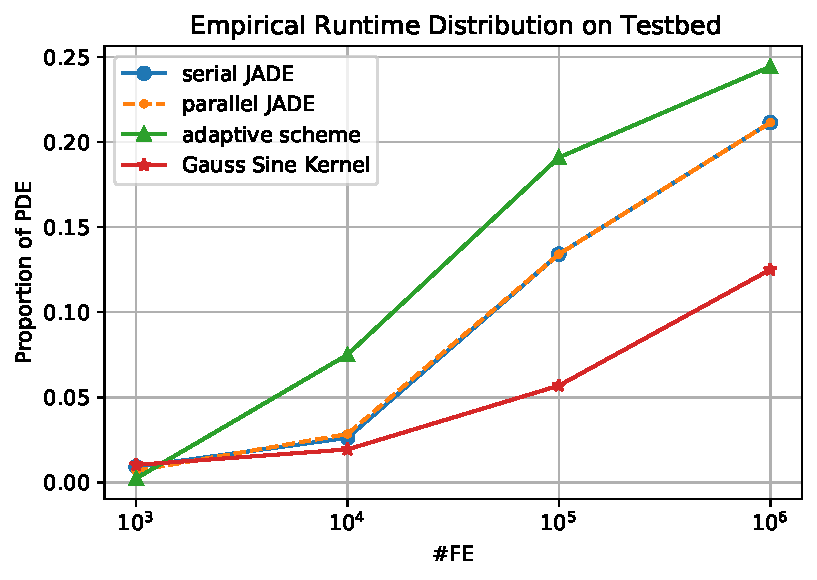
\includegraphics[width=\textwidth]{../../code/experiments/misc/ert_plot.pdf}
	}
	\unterschrift{Empirical Runtime Distribution of all algorithms on the 11 testbed \gls{pde}s at target values $5\cdot 10^{-2}$, $1\cdot 10^{-2}$, $5\cdot 10^{-3}$ and $1\cdot 10^{-3}$.}{}{}
	\label{fig:ert_plot}
\end{figure}
Remarkable is the virtually non-existing performance difference between the serial and the parallel memetic JADE. The adaptive JADE scores continuously best and solves up to a quarter of the target values. This is largely thanks to the good performance on \gls{pde} 0A, which contributes 9 percent $\left( \frac{1}{11} \right)$ to the whole testbed. Extrapolating the \gls{erd} plots indicates a further performance increase with more \gls{nfe}. Due to the already expensive algorithm, this is not tested. 

\end{document}